\documentclass[letterpaper,pdftex]{article}

\setlength{\textwidth}{168mm}
\setlength{\textheight}{210mm}
\setlength{\oddsidemargin}{0cm}
\setlength{\topmargin}{0cm}
\setlength{\headheight}{48pt}
\addtolength{\textheight}{-25pt}
\voffset -0.5in

\usepackage{natbib}
\usepackage[utf8]{inputenc}
\usepackage[english]{babel}
\usepackage{xcolor,graphicx}
\usepackage{fancyhdr}
\usepackage{multirow}
\usepackage{siunitx}
\usepackage{hyperref}
\hypersetup{
    colorlinks,
    citecolor=blue,
    filecolor=black,
    linkcolor=blue,
    urlcolor=black
}
\usepackage{epstopdf}
\usepackage[autolinebreaks,useliterate]{mcode}
\pagestyle{fancy}
\renewcommand{\headrule}{\color{gray}
\hrule width\headwidth height\headrulewidth \vskip-\headrulewidth}
\renewcommand{\footrule}{{\color{gray}
\vskip-\footruleskip\vskip-\footrulewidth
\hrule width\headwidth height\footrulewidth\vskip\footruleskip}}
\renewcommand{\headrulewidth}{1.5pt}
\renewcommand{\footrulewidth}{1.5pt}

\usepackage{caption}
\usepackage{subcaption}


\begin{document}
\fancyhead{}
\fancyfoot{}
\fancyhead[L]{
\begin{minipage}{3.5cm}
\begin{center}
	
\includegraphics[width=0.95\textwidth]{logousb.png}
\end{center}
\end{minipage}
\begin{minipage}{12cm}
\begin{flushleft}
\small \textsc{Universidad de San Buenaventura}\\
\small \textsc{School of Engineering}\\
\small \textsc{Mechatronics Engineering\\}
\end{flushleft}
\end{minipage}
}
\fancyhead[R]{
\begin{minipage}{3.0cm}
\begin{flushright}
\small \textsc{Mechanics of Materials \\ 3rd Term}\\
\small \textsc{2021-I}
\end{flushright}
\end{minipage}
}
\fancyfoot[R]{\large \textbf{\thepage}}

\begin{minipage}{0.3\textwidth}
\begin{flushleft}
\textbf{Author:}\\
\textit{Nikolay Prieto Ph.D(c)}\\
\end{flushleft}
\end{minipage}
\begin{minipage}{0.7cm}
\textcolor{gray}{\rule{0.3cm}{2.5cm}}
\end{minipage}
\begin{minipage}{0.64\textwidth}
\Large{\textbf{Computational Laboratory \\ ANSYS (Part II \\ Elelements and Meshes)}}
\end{minipage}\\

\noindent
\textcolor{gray}{\rule{\textwidth}{0.5pt}}\\
\renewcommand{\tablename}{Tabla}
\renewcommand{\arraystretch}{1.2}
\renewcommand\contentsname{Outline}
\tableofcontents

\noindent
\textcolor{gray}{\rule{\textwidth}{0.5pt}}\\

\section{Introduction}

In the previous laboratory, we discussed some of the assumptions that can be used to simplify and reduce the dimensionality of a Finite Element Model (FEM). For example, if a beam has a constant cross section, it can be modeled as a one-dimensional body. If a beam is symmetric with a uniform cross section, it can be modeled as a two-dimensional body. Or, it can be modeled as three dimensional body. If created correctly, all three types of models will produce the same results. However, they will have different solid model geometry and must be meshed using different element types (Fig. \ref{fig:cantilever} )

\begin{figure}[h]
   \centering
   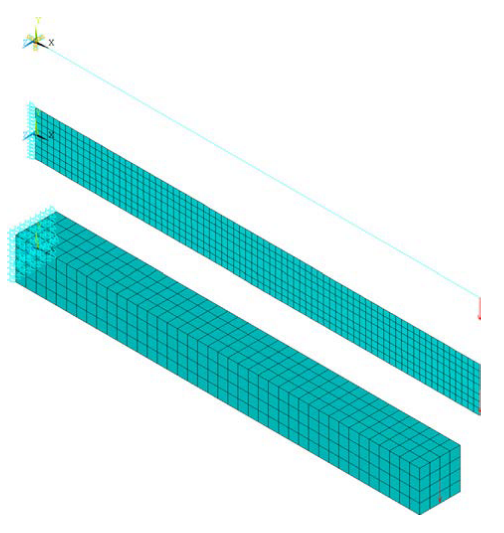
\includegraphics[width=0.6\textwidth]{cantileverbeam}
   \caption{Element Plots of a Square Cantilever Beam Modeled using 1D Beam Elements (BEAM189, top), 2D Continuum Elements (PLANE183, center), and 3D Continuum Elements (SOLID185, bottom).}
   \label{fig:cantilever}
\end{figure}

\section{Elements}

The Ansys library element is available to be used dependent on the purpose. There are specific elements for heat transfer, static structural, fluid dynamics or transient (time domain) problems. Each ANSYS element has a number of properties including its name, characteristic and degen- erate shapes, number of nodes, degrees of freedom, real constants, key options, material properties, permitted loads, and special features. An overview of these features can be found in the input summary of each element in the ANSYS Element Library. The input summary follows the element description and the element input data.

Each element in ANSYS has a name followed by a number. The combination of a name and a number cannot exceed 8 characters. The name indicates the element’s family (FLUID, PLANE, SHELL, SOLID, etc.). The number is a unique identifier called the element routine number. For example, a PLANE182 element is a member of the PLANE element family and it is element routine number 182. When element types are defined using the command line or input files, only the routine number is required. The element family name is optional.

\subsection{Element shapes}

There are eight possible element shapes in ANSYS: points (for point elements); lines (for line elements); triangles or quadrilaterals (for area elements); and tetrahedrons, pyramids, prisms, or bricks (for volume elements). These shapes are shown in Fig. \ref{fig:shapes}

\begin{figure}[h]
   \centering
   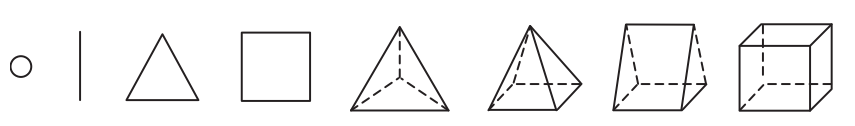
\includegraphics[width=0.95\textwidth]{elementshapes}
   \caption{Possible Element Shapes in ANSYS.}
   \label{fig:shapes}
\end{figure}

\subsection{Number of nodes}

All elements have nodes that define their location in space. For example, quadrilateral elements like PLANE55 have four nodes (I, J, K, and L)—one for each corner (Fig. \ref{fig:nodes}, left). For example, PLANE77 is the counterpart to PLANE55 with midside nodes. It has a total of eight nodes (I, J, K, L, M, N, O and P) - one for each corner and one in the middle of each side (Figure \ref{fig:nodes}, right). The node letters refer to the position of the nodes on a generic element (i.e., on the element type). The node lettering convention starts with the letter I and increments one letter per node.

\begin{figure}[h]
   \centering
   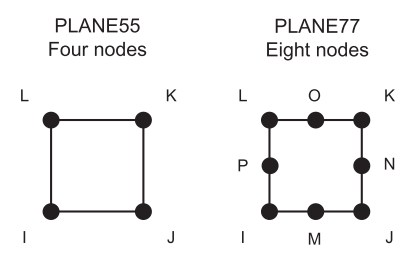
\includegraphics[width=0.6\textwidth]{nodesinelement}
   \caption{Quadrilateral Elements Without and With Mid-Side Nodes.}
   \label{fig:nodes}
\end{figure}

Quadrilateral and brick elements can be forced into degenerate shapes with one or more triangular faces in order to mesh geometries that could not be meshed otherwise. For example, a quadrilateral element may collapse into a triangle (Figure 4.7, \ref{fig:nodes_elements}), while a brick element may collapse into a prism, a pyramid, or a tetrahedron. This is achieved by defining the same node number for multiple nodes (Figure \ref{fig:nodes_elements}, right).

\begin{figure}[h]
   \centering
   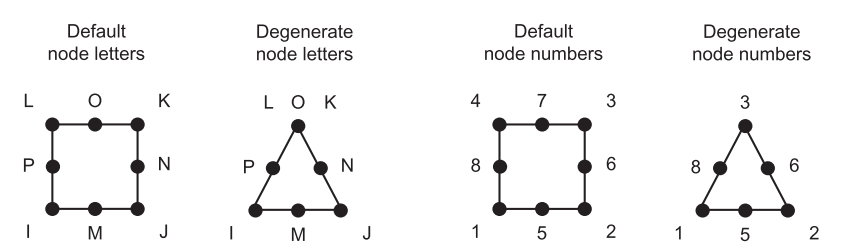
\includegraphics[width=0.9\textwidth]{shapesandnodes}
   \caption{Quadrilateral Elements with Default and Degenerate Shapes: Node Letters for a Generic Element (left) and Node Numbers for a Specific Element in a FE Mesh (right)}
   \label{fig:nodes_elements}
\end{figure}

\subsection{Degrees of freedom}

The degrees of freedom (DOFs) are the primary unknowns in the equations that constitute a FEM. Solving the equations determines the values of the DOFs for each node in the model. These values are referred to as the ''primary data'' in the documentation. The derived data (stresses, strains, gradients, fluxes, etc.) are calculated from the DOF solution. ANSYS DOFs include displacements (UX, UY, UZ), rotations (ROTX, ROTY, ROTZ), temperature (TEMP), fluid pressure (PRES), fluid kinetic energy (ENKE), magnetic vector potential (AX, AY, AZ), voltage (VOLT), and current (CURR). As an example Figs. \ref{fig:structuralDOF} and \ref{fig:thermalDOF} show the DOF of some ANSYS elements for structural and thermal analysis, respectively.

\begin{figure}[h]
   \centering
   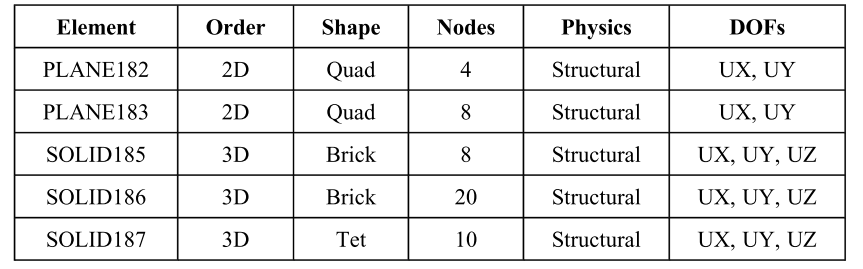
\includegraphics[width=0.9\textwidth]{StructuralDOF}
   \caption{Commonly Used Structural Continuum Elements}
   \label{fig:structuralDOF}
\end{figure}

\begin{figure}[h]
   \centering
   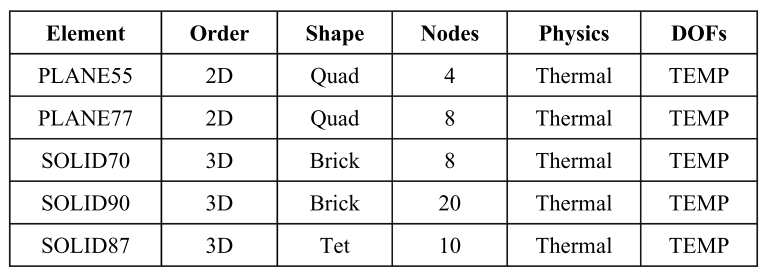
\includegraphics[width=0.9\textwidth]{thermalDOF}
   \caption{Commonly Used Thermal Continuum Elements}
   \label{fig:thermalDOF}
\end{figure}

The degrees of freedom included in each element type reflect the physics of the underlying problem. You should choose elements that offer only the degrees of freedom that you require since additional degrees of freedom increase computation time and provide no benefit. For example, structural analysis does not (usually) involve heat transfer or voltages. Therefore, the element(s) used to model structures should not have TEMP or VOLT DOFs.


\section{Practical Exercises}

In this laboratory, you will perform a steady-state structural analysis of a cantilever beam using 1D, 2D, and 3D models meshed with beam, plane, and solid elements. The beam is made of aluminum with a Young’s modulus of $73.1$GPa and a Poisson’s ratio of $0.33$. It is $1.0$m in length with a $100\times100$mm cross section. It has a load of $5000$N applied to the unsupported end (Figure \ref{fig:problem}). 

The 1D model will be meshed with BEAM189 elements. The 2D model will be meshed with PLANE182 elements. And, the 3D model will be meshed with SOLID186 elements. The goal of each analysis is to determine the deflection at the end of the beam and the stresses throughout the beam. Once all three models have been solved, the differences and similarities among the results of the three models will be examined.

\begin{figure}[h]
   \centering
   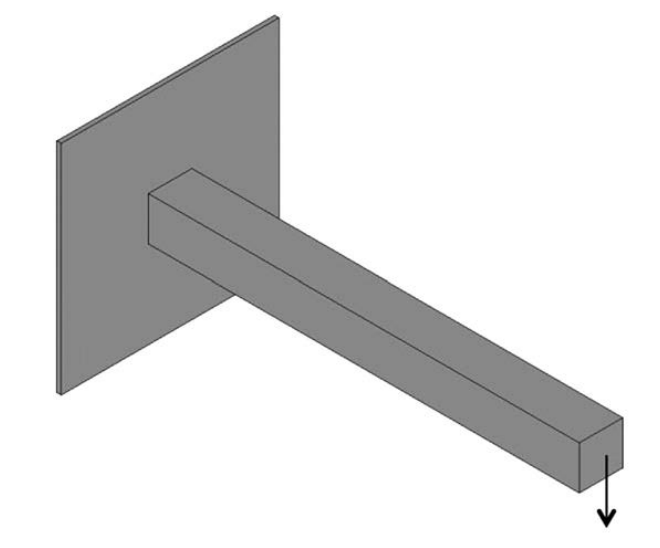
\includegraphics[width=0.5\textwidth]{problem}
   \caption{Schematic of Cantilever Beam with End Load.}
   \label{fig:problem}
\end{figure}

\subsection{Material properties}
\begin{itemize}
\item Young's Modulus $7.310\times10^{10}$Pa
\item Poisson's ratio $0.33$
\end{itemize}
\subsection{Boundary Conditions}
\begin{itemize}
\item $6000$ N downward load applied to the center of the free end of the beam
\item The fixed end of the beam is fully constrained in x, y, and z.
\end{itemize}

\section{Report content}
\begin{itemize}
\item The report should be formatted as a IEEE template style.
\item The report may content the following sections: Abstract, Introduction, Methods, Results, Discussion and Conclusions.
\item Do not forget to perform the analysis in 1D, 2D and 3D. 
\item Apply the element types mentioned.
\item Implement a convergence analysis for each dimension, you can plot it as shown in Fig. \ref{fig:convergence}. For each dimension problem implement the following ranges in quantity of elements: $elem=[100,1000,5000,10000,50000]$
\item Perform the analytical method (pure bending)
\item Make a table with the main results on each and compare with the analytical answer, as shown in Fig. \ref{fig:tableresults}
\item Do not forget to establish strong conclusions. 
\end{itemize}

\begin{figure}[h]
   \centering
   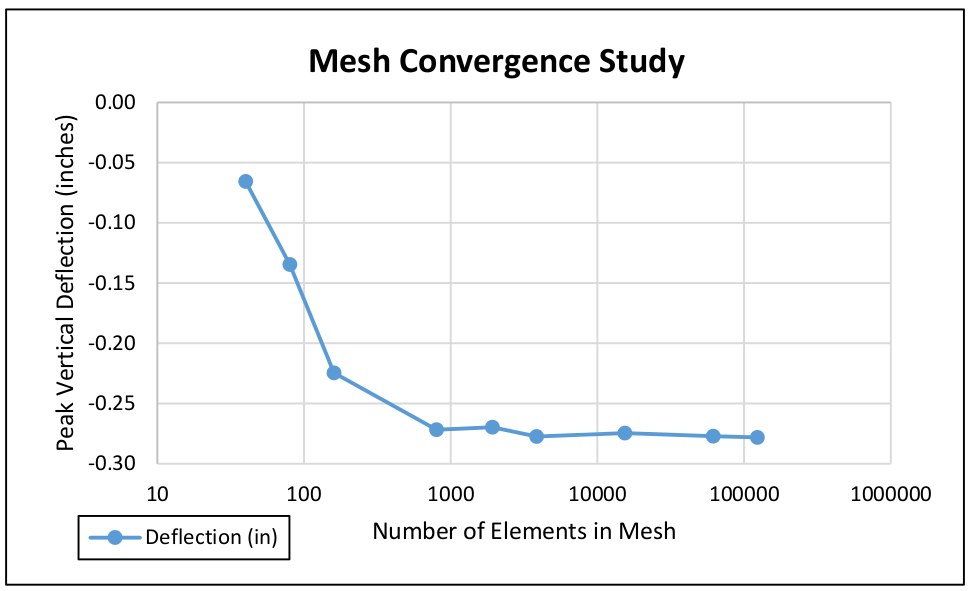
\includegraphics[width=0.7\textwidth]{Mesh-Convergence}
   \caption{Example of a mesh convergence plot.}
   \label{fig:convergence}
\end{figure}

\begin{figure}[h]
   \centering
   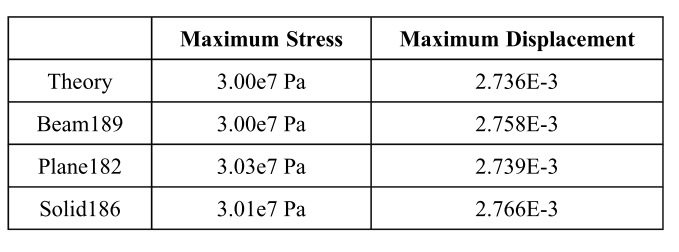
\includegraphics[width=0.7\textwidth]{tableresults}
   \caption{Example of general results plot.}
   \label{fig:tableresults}
\end{figure}

This laboratory is inspired from the book of \cite{Thompson2017}. Enjoy this lab, regards!


\bibliographystyle{apalike}

\bibliography{Referencias.bib}


\end{document}